\subsection{The Slope of a Line}\pp

 {\tmstrong{Objective: Find the slope of a line given a graph or two points.}}\pp

 As we graph lines, we will want to be able to identify different properties of
the lines we graph. One of the most important properties of a line is its
slope. {\tmstrong{Slope}} is a measure of steepness. A line with a large
slope, such as 25, is very steep. A line with a small slope, such as
$\frac{1}{10}$ is very flat. We will also use slope to describe the direction
of the line. A line that goes up from left to right will have a positive slope
and a line that goes down from left to right will have a negative slope.\pp

 As we measure steepness we are interested in how fast the line rises compared
to how far the line runs. For this reason we will describe slope as the
fraction $\frac{\tmop{rise}}{\tmop{run}}$. Rise would be a vertical change, or
a change in the $y$-values. Run would be a horizontal change, or a change in
the $x$-values. So another way to describe slope would be the fraction
$\frac{\tmop{change} \tmop{in} y}{\tmop{change} \tmop{in} x}$. It turns out
that if we have a graph we can draw vertical and horiztonal lines from one
point to another to make what is called a slope triangle. The sides of the
slope triangle give us our slope. The following examples show graphs that we
find the slope of using this idea.

\begin{example}\label{Lin46}
~\end{example}  
  \begin{multicols}{2}
    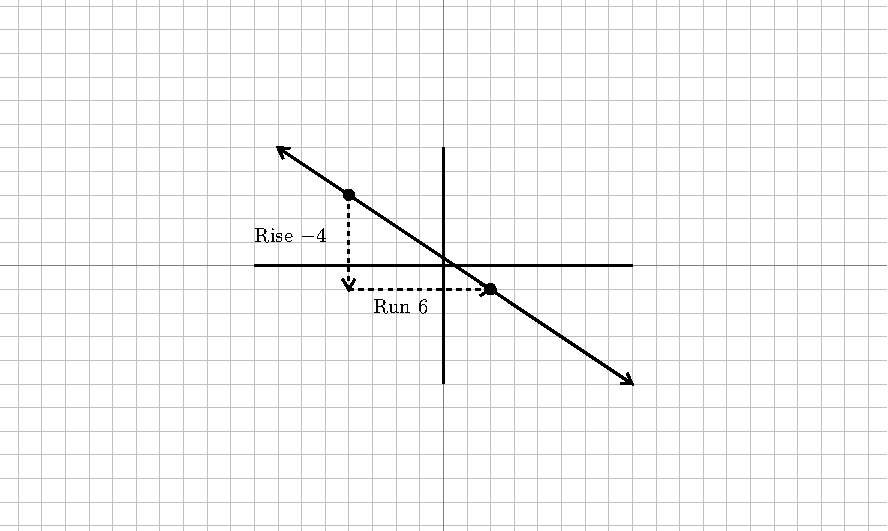
\includegraphics[scale=.9,bb = 115 65 310 190, clip=true]{II_1_3c-1.eps}
    
    \
    
    To find the slope of this line we will consider the rise, or vertical
    change and the run or horizontal change. Drawing these lines in makes a
    slope triangle that we can use to count from one point to the next the
    graph goes down 4, right 6. This is rise $- 4$, run 6. As a fraction it
    would be, $\frac{- 4}{6}$. Reduce the fraction to get $\frac{-2}{3}$.
  \end{multicols}
\begin{center}
A slope of $-\displaystyle\frac{2}{3}$ is our solution.
\end{center}%\end{example}
~\par
 {\tmstrong{World View Note: }}When French mathematicians Rene Descartes and
Pierre de Fermat first developed the coordinate plane and the idea of graphing
lines (and other functions) the $y$-axis was not a vertical line!\pp

\begin{example}\label{Lin47}
~\end{example}  
 \begin{multicols}{2}
    \includegraphics[scale=.9,bb = 115 65 310 190, clip=true]{II_1_3c-2.eps}
    
    To find the slope of this line, the rise is up 6, the run is right 3.\pp
		Our slope is then written as a fraction, $\frac{\tmop{rise}}{\tmop{run}}$ or
    $\frac{6}{3}$.\pp
		This fraction reduces to 2.  This will be our slope.
		  \end{multicols}
  %\begin{eqnarray*}
\begin{center}
A slope of $2$ is our solution.
\end{center}
  %\end{eqnarray*}
%\end{example}

 There are two special lines that have unique slopes that we need to be aware
of. They are illustrated in the following example.

\begin{example}\label{Lin48}
~\end{example}
  \begin{multicols}{2}
    \includegraphics[scale=.9,bb = 115 65 310 190, clip=true]{II_1_3c-3.eps}
    
    In this graph there is no rise, but the run is 3 units. This slope becomes
    
    $\frac{0}{3} = 0$. \tmop{This} \tmop{line}, \tmop{and} \tmop{all}
    \tmop{horizontal} \tmop{lines} \tmop{have} a \tmop{zero} \tmop{slope}.
    
%    \ $
    
    \includegraphics[scale=.9,bb = 115 65 310 190, clip=true]{II_1_3c-4.eps}
    
    This line has a rise of 5, but no run. The slope becomes $\frac{5}{0} =$
    \tmop{undefined}. \tmop{This} \tmop{line}, \tmop{and} \tmop{all}
    \tmop{vertical} \tmop{lines}, \tmop{have} \tmop{no} \tmop{slope}.
  \end{multicols}
%\end{example}

 As you can see there is a big difference between having a zero slope and
having no slope or undefined slope. Remember, slope is a measure of steepness.
The first slope is not steep at all, in fact it is flat. Therefore it has a
zero slope. The second slope can't get any steeper. It is so steep that there
is no number large enough to express how steep it is. This is an undefined
slope.\pp

 We can find the slope of a line through two points without seeing the points
on a graph. We can do this using a slope formula. If the rise is the change in
$y$ values, we can calculate this by subtracting the $y$ values of a point.
Similarly, if run is a change in the $x$ values, we can calculate this by
subtracting the $x$ values of a point. In this way we get the following
equation for slope.\pp

%\bbm
{\tmstrong{
\[ \tmop{The} \tmop{slope} \tmop{of} \tmop{a} \tmop{line} \tmop{through~} (x_1, y_1)
   \tmop{~and~} (x_2, y_2) \tmop{~is~} \frac{y_2 - y_1}{x_2 - x_1}. \]}}
%\ebm

 When mathematicians began working with slope, it was called the modular slope.
For this reason we often represent the slope with the variable $m$. Now we
have the following for slope.\pp

\bbm
\[ \tmmathbf{\tmop{Slope} = m = \frac{\tmop{rise}}{\tmop{run}} =
   \frac{\tmop{change} \tmop{in} y}{\tmop{change} \tmop{in} x} = \frac{y_2 -
   y_1}{x_2 - x_1}} \]
\ebm 
\pp
As we subtract the $y$ values and the $x$ values when calculating slope it is
important we subtract them in the same order. This process is shown in the
following examples.

\begin{example}\label{Lin49}
  
  \begin{eqnarray*}
    \tmop{Find} \tmop{the} \tmop{slope} \tmop{between} (- 4, 3) \tmop{~and~} (2,
    - 9) &  & \tmop{Identify} x_1, y_1, x_2, y_2\\
    (x_1, y_1) \tmop{~and~} (x_2, y_2) &  & \tmop{Use} \tmop{slope}
    \tmop{formula}, m = \frac{y_2 - y_1}{x_2 - x_1}\\
    m = \frac{- 9 - 3}{2 - (- 4)} &  & \tmop{Simplify}\\
    m = \frac{-12}{6} &  & \tmop{Reduce}\\
    m = - 2 &  & \tmop{Our} \tmop{solution}
  \end{eqnarray*}
\end{example}

\begin{example}\label{Lin50}
  \begin{eqnarray*}
    \tmop{Find} \tmop{the} \tmop{slope} \tmop{between} (4, 6) \tmop{~and~} (2, -
    1) &  & \tmop{Identify} x_1, y_1, x_2, y_2\\
    (x_1, y_1) \tmop{~and~} (x_2, y_2) &  & \tmop{Use} \tmop{slope}
    \tmop{formula}, m = \frac{y_2 - y_1}{x_2 - x_1}\\
    m = \frac{- 1 - 6}{2 - 4} &  & \tmop{Simplify}\\
    m = \frac{- 7}{- 2} &  & \tmop{Reduce}, \tmop{dividing} \tmop{by} - 1\\
    m = \frac{7}{2} &  & \tmop{Our} \tmop{solution}
  \end{eqnarray*}
\end{example}

 We may come up against a problem that has a zero slope (horizontal line) or no
slope (vertical line) just as with using the graphs.

\begin{example}\label{Lin51}
  
  \begin{eqnarray*}
    \tmop{Find} \tmop{the} \tmop{slope} \tmop{between~} (- 4, - 1) \tmop{~and~}
    (- 4, - 5) &  & \tmop{Identify} x_1, y_1, x_2, y_2\\
    (x_1, y_1) \tmop{~and~} (x_2, y_2) &  & \tmop{Use} \tmop{slope}
    \tmop{formula}, m = \frac{y_2 - y_1}{x_2 - x_1}\\
    m = \frac{- 5 - (- 1)}{- 4 - (- 4)} &  & \tmop{Simplify}\\
    m = \frac{- 4}{0} &  & \tmop{Can' t} \tmop{divide} \tmop{by} \tmop{zero}\\
    \tmop{Slope} m \tmop{is~undefined} &  & \tmop{Our} \tmop{solution}
  \end{eqnarray*}
\end{example}

\begin{example}\label{Lin52}
  \begin{eqnarray*}
    \tmop{Find} \tmop{the} \tmop{slope} \tmop{between~} (3, 1) \tmop{~and~} (- 2,
    1) &  & \tmop{Identify} x_1, y_1, x_2, y_2\\
    (x_1, y_1) \tmop{~and~} (x_2, y_2) &  & \tmop{Use} \tmop{slope}
    \tmop{formula}, m = \frac{y_2 - y_1}{x_2 - x_1}\\
    m = \frac{1 - 1}{- 2 - 3} &  & \tmop{Simplify}\\
    m = \frac{0}{- 5} &  & \tmop{Reduce}\\
    m = 0 &  & \tmop{Our} \tmop{solution}
  \end{eqnarray*}
\end{example}

 Again, there is a big difference between no slope and a zero slope. Zero is an
integer and it has a value, the slope of a flat horizontal line. No slope has
no value, it is undefined, the slope of a vertical line.\pp

 Using the slope formula we can also find missing points if we know what the
slope is. This is shown in the following two examples.

\pagebreak

\begin{example}\label{Lin53}~~
%~\pp
 Find the value of $y$ between the points (2, $y$) \tmop{~and~} \\(5, - 1) with
  slope $- 3$.\\
  \begin{eqnarray*}
    m = \frac{y_2 - y_1}{x_2 - x_1} &  & \tmop{We} \tmop{will} \tmop{plug}
    \tmop{values} \tmop{into~the} \tmop{slope} \tmop{formula}\\
    - 3 = \frac{- 1 - y}{5 - 2} &  & \tmop{Simplify}\\
    - 3 = \frac{- 1 - y}{3} &  & \tmop{Multiply} \tmop{both} \tmop{sides}
    \tmop{by} 3\\
    - 3 {\bf(3)} = \frac{- 1 - y}{3} {\bf(3)} &  & \tmop{Simplify}\\
    - 9 = - 1 - y &  & \tmop{Add} 1 \tmop{to} \tmop{both} \tmop{sides}\\
    \bf{\underline{+ 1 ~~~+ 1}}~~~~  &  & \\
    - 8 = - y &  & \tmop{Divide} \tmop{both} \tmop{sides} \tmop{by} - 1\\
    \bf{\overline{- 1} ~~~~ \overline{- 1}} &  & \\
    8 = y &  & \tmop{Our} \tmop{solution}
  \end{eqnarray*}
\end{example}

%\pagebreak

\begin{example}\label{Lin54}~~
%~\pp 
Find the value of $x$ between the points (- 3, 2) \tmop{~and~} \\($x$, 6) with
  slope $\displaystyle\frac{2}{5}$.\\
  \begin{eqnarray*}
    m = \frac{y_2 - y_1}{x_2 - x_1} &  & \tmop{We} \tmop{will} \tmop{plug}
    \tmop{values} \tmop{into} \tmop{slope} \tmop{formula}\\
    \frac{2}{5} = \frac{6 - 2}{x - (- 3)} &  & \tmop{Simplify}\\
    \frac{2}{5} = \frac{4}{x + 3} &  & \tmop{Multiply} \tmop{both}
    \tmop{sides} \tmop{by~} (x + 3) \\
    \frac{2}{5} (x + 3) = 4 &  & \tmop{Multiply} \tmop{by} 5 \tmop{to}
    \tmop{clear} \tmop{fraction}\\
    {\bf(5)} \frac{2}{5} (x + 3) = 4 {\bf(5)} &  & \tmop{Simplify}\\
    2 (x + 3) = 20 &  & \tmop{Distribute}\\
    2 x + 6 = 20 &  &  \\
    \bf{\underline{- 6 ~~- 6}} &  & \tmop{Subtract} 6 \tmop{from} \tmop{both}
    \tmop{sides}\\
    2 x = 14 &  & \tmop{Divide} \tmop{each} \tmop{side} \tmop{by} 2\\
    \bf{\overline{2} ~~~~~ \overline{2}}~ &  & \\
    x = 7 &  & \tmop{Our} \tmop{solution}
  \end{eqnarray*}
\end{example}